\chapter{Feature Extraction}

\section{Overview of Feature Extraction}
For a single experiment data, i.e., a single fruit fly recorded between ZT10 and ZT2 (zeitgeber time 10 and 2), feature extraction consists of four consecutive steps,  where the input in one stage is the output of the previous one.
The input of the first step is the raw output signal of the tracking and pose estimation model; in our case, the output of DeepLabCut, a toolbox for markerless pose estimation.
The feature extraction steps are as follows:

\begin{enumerate}
	\item Constructing pose values and preprocessing; dealing with occluded body parts, alignment of different orientations, filtering, and imputation.
	\item Computing spatio-temporal features, such as distances between body parts, velocity, and angular velocity from body part positions.
	\item Computing dynamic postural features by extending spatio-temporal features to multiple timescales using wavelet transformation and sliding window statistics.
	\item Computing normalized high-dimensional behavioral representations.
\end{enumerate}

Matrices $\V{X} \in \mathbb{R}^{T \times N}$ and $\V{Y} \in \mathbb{R}^{T \times N}$ denotes a multivariate time series for $x$ and $y$ cartesian components of two-dimensional video recordings that are collected for $N$ tracked body parts of the fly on $T$ consecutive time stamps by a pose estimation model.
This multivariate time series matrices $\V{X}$ and $\V{Y}$ are the raw input data that goes into the first step of the feature extraction.
Note that the number of body parts, $N$, must be the same among all experiments conducted with different fruit flies, but the number of time stamps, $T$, might differ.
Each column of the $\V{X}=\qmatrix{\V{x}_1, \cdots, \V{x}_N}^\top$ and $\V{Y}=\qmatrix{\V{y}_1, \cdots, \V{y}_N}^\top$ can be written respectively as follows:
\begin{equation}
	\begin{aligned}
		\V{y}_i & = (y_{i,1}, y_{i,2}, \dots, y_{i,t-1}, y_{i,t}, y_{i,t+1}, \dots, y_{i,T}), \\
		\V{x}_i & = (x_{i,1}, x_{i,2}, \dots, x_{i,t-1}, x_{i,t}, x_{i,t+1}, \dots, x_{i,T}).
	\end{aligned}
\end{equation}

Here $i$ denotes the index of the body part, e.g., leg tip or proboscis.

In addition to $\V{X}$ and $\V{Y}$, a pose estimation model may report prediction scores for each tracked body part at each time step, which is the case for DeepLabCut as well.
$L \in \mathbb{R}^{N \times T}$ denotes the time series of prediction scores, each column of the $L=[\V{l_1}, \cdots, \V{l_N}]^\top$ can be written as follows:

\begin{equation}
	\V{l}_i = (l_{i,1}, l_{i,2}, \dots, l_{i,t-1}, l_{i,t}, l_{i,t+1}, \dots, l_{i,T}).
\end{equation}

The prediction scores tend to be very low when the body part is not visible.
Thus, $L$ provides valuable information about the occluded body parts.
In the Section~\ref{section:dealing-with-occluded-body-parts}, how $L$ is incorporated into construction of pose values is described in detail.

\section{Preprocessing}
This step involves preprocessing the signal by filtering and imputation of certain video frames.
But in addition to this, there are a couple of optional procedures that can be beneficial for our task of learning stereotypical behaviors.
These additional procedures deal with occluded body parts of the fly, alignment of the fly orientations and defining new points of interest.

\subsection{Occluded Body Parts}\label{section:dealing-with-occluded-body-parts}
As mentioned in the Section~\ref{section:challanges}, the two-dimensionality of the video recordings introduces several significant challenges,  one of which is the occluded body parts.
There are many types of occlusions. One type is short occlusions that often results from postural changes. Imputation of the time series $\V{X}$ and $\V{Y}$ for such short occlusions is relatively easy since the number of consecutive missing data points is few.
However, this is not the case for long occlusions, which usually occur when the fly is dormancy for an extended period of time.
Especially for the body parts with left and right counterparts, fly's orientation can result in one of the counterparts being occluded for long dormancy epochs.
We use imputation and elimination of corresponding data-points to deal with the occlusions. Before describing those approaches, we define a criterion for being occluded.

\subsubsection{Oriented Pose Values for Body Parts with Left \& Right Counterparts}\label{section:oriented-pose-values}
If the fly is oriented perpendicular to the camera perspective, as in Figure~\ref{figure:perpendicular-orientation}, then one of the left and right body parts is often occluded.
In other orientations (e.g., Figure~\ref{figure:parallel-horizontal-orientation} and Figure~\ref{figure:oblique-orientation}),  both of them or none of them might be occluded as well.
However, in the conducted experiments, flies usually choose to stay dormancy perpendicular to the camera perspective in long dormancy epochs, as mentioned in Chapter~\ref{chapter:expt-data-collection}.
In such cases, one can concede using only one of the left and right counterparts to construct pose values.
Therefore, this optional step is included in the behavioral mapping pipeline to reduce pose values of body parts with left and right counterparts to a single value.

\begin{figure}[ht!]
	\centering
	\begin{subfigure}[b]{0.325\linewidth}
		\centering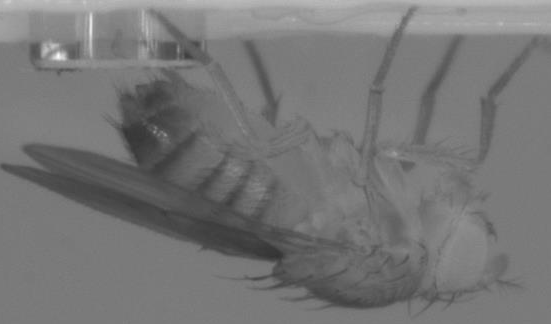
\includegraphics[width=\linewidth]{figures/FlyOrientation-ParallelHorizontal.png}
		\caption{Parallel.\label{figure:parallel-horizontal-orientation}}
	\end{subfigure}%
	% \hfill
	% \centering
	% \begin{subfigure}[ht!]{0.24\linewidth}
	% 	\centering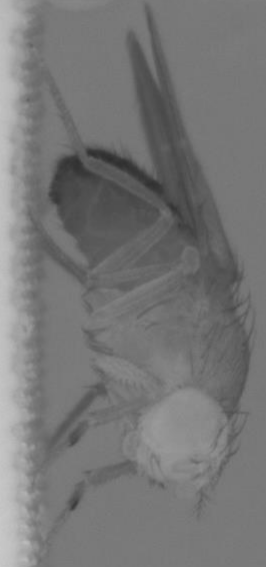
\includegraphics[width=\linewidth]{figures/FlyOrientation-ParallelVertical.png}
	% 	\caption{\label{figure:parallel-vertical-orientation}}
	% \end{subfigure}%
	\hfill
	\begin{subfigure}[b]{0.3\linewidth}
		\centering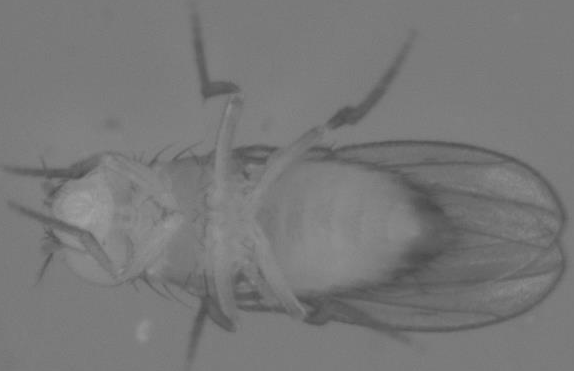
\includegraphics[width=\linewidth]{figures/FlyOrientation-Oblique.png}
		\caption{Oblique.\label{figure:oblique-orientation}}
	\end{subfigure}%
	\hfill
	\begin{subfigure}[b]{0.3\linewidth}
		\centering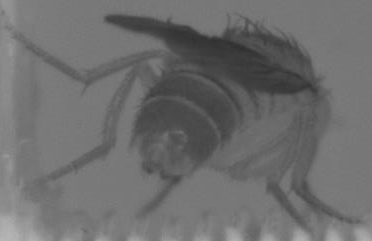
\includegraphics[width=\linewidth]{figures/FlyOrientation-Perpendicular.png}
		\caption{Perpendicular.\label{figure:perpendicular-orientation}}
	\end{subfigure}
	\caption[Three examples demonstrating the different orientations viewed by the camera.]    {Three examples demonstrating the different orientations viewed by the camera. Orientations similar to Figure~\ref{figure:oblique-orientation} and Figure~\ref{figure:perpendicular-orientation} results in occluded body parts and hence erroneous tracking.}
\end{figure}

We use prediction scores to determine which body part should be used to compute oriented pose values.
Let $i$ and $j$ be a pair of body parts which are left and right counterparts of each other, e.g., left haltere and right haltere.
Then, one can use the $\V{l}_i$ and $\V{l}_j$ to predict if one of them is occluded at a particular time step $t$.
Let $\orient{\V{x}_i, \V{x}_j}$ ($\orient{\V{y}_i, \V{y}_j}$) be a new pose vector that will be computed based on $\V{x}_i$ and $\V{x}_j$ ($\V{y}_i$ and $\V{y}_j$), e.g., a vector of oriented haltere pose values, composed of left haltere and right haltere pose values.
The following conditional procedures are proposed to compute oriented pose values from the left and right pose values by deciding the orientation of the fly for a counterpart body pair. The procedures below can be used separately, or successively.

\begin{itemize}
	\item If $l_{i,t} - l_{j,t} \geq  \epsilon$, then, without loss of generality, $\orient{\V{x}_i, \V{x}_j}_t=x_{i,t}$ and $\orient{\V{y}_i, \V{y}_j}_t=y_{i,t}$ for a threshold $\epsilon$, typically $\epsilon > 0.5$.

	\item If $\card*{\Set{t^{\prime}}{l_{i,t^{\prime}} > l_{j,t^{\prime}}, \, t^{\prime} \in [t-\tau \rangedots t+\tau]}} > \tau$, then, without loss of generality, $\orient{\V{x}_i, \V{x}_j}_t=x_{i,t}$ and $\orient{\V{y}_i, \V{y}_j}_t=y_{i,t}$, for a window of size $2w+1$.

	\item If $l_{i,t} > l_{j,t}$ and if the nearest confident left orientation is closer than the nearest confident right orientation, i.e., $$\argmin_{t^{\prime}} \Set{\abs*{t-t^{\prime}}}{l_{i,t^{\prime}} - l_{j,t^{\prime}} \geq \epsilon} > \argmin_{t^{\prime}} \Set{\abs*{t - t^{\prime}}}{l_{j,t^{\prime}} - l_{i,t^{\prime}} \geq \epsilon},$$ then, without loss of generality, $\orient{\V{x}_i, \V{x}_j}_t=x_{i,t}$ and $\orient{\V{y}_i, \V{y}_j}_t=y_{i,t}$.
	\item If simply $l_{i,t} > l_{j,t}$, then without loss of generality, $\orient{\V{x}_i, \V{x}_j}_t=x_{i,t}$ and $\orient{\V{y}_i, \V{y}_j}_t=y_{i,t}$.
\end{itemize}

Except directly comparing the prediction confidence scores as in the last procedure, some of the time points might be left with undecided orientations.
If the number of such time points is acceptable, then directly comparing the prediction scores for those time points is convenient and handy.

After applying the above procedures for a left and right counterpart pair $i$ and $j$, we can define oriented multivariate time series as
\begin{equation}
	\begin{aligned}
		\V{X}^{\omicron} & = \rbr{\qmatrix{\rbr{\V{x}_k}_{k \notin \bigcup_{\set{i,j} \in \mathcal{O}} \set{i,j}}}^\top \concat \qmatrix{\rbr{\orient{\V{x}_i, \V{x}_j}}_{\set{i,j} \in \mathcal{O}}}^\top}, \\
		\V{Y}^{\omicron} & = \rbr{\qmatrix{\rbr{\V{y}_k}_{k \notin \bigcup_{\set{i,j} \in \mathcal{O}} \set{i,j}}}^\top \concat \qmatrix{\rbr{\orient{\V{y}_i, \V{y}_j}}_{\set{i,j} \in \mathcal{O}}}^\top},
	\end{aligned}
\end{equation}
where $\mathcal{O}$ is the set of index pairs of left and right counterparts and $\bigcup_{\set{i,j} \in \mathcal{O}} \set{i,j}$ is the union of all indexes of such body parts pairs.
Applying described procedures for each left and right counterparts results in computing $\V{X}^{\omicron}$ and $\V{Y}^{\omicron}$.
This oriented versions of original data matrices can be used instead of $\V{X}$ and $\V{Y}$ in the rest of the pipeline, if desired.

\subsubsection{Detecting Occlusions Using Prediction Scores \& Anomalous Pose Values}\label{section:detecting-occlusions}
Major postural changes and overlapping body parts during movements result in some body parts being occluded for a short interval of time.
These types of occlusions may span several frames to several seconds.
Since the pose estimation model makes predictions for such data points, it is necessary to detect and process such data points.
Our pipeline exploits two indicators for detection: prediction scores and anomalous changes in pose values.
We mark the body parts estimated to be occluded and corresponding time intervals, and then the desired imputation method is used to fill those time intervals appropriately.

The following conditions are considered to detect occluded body parts, note that they can be used separately or in combination with each other.
\begin{itemize}
	\item If the prediction confidence score at time step $t$ is lower than a given threshold $\epsilon$, then the $t$ is marked to be imputed.
	\item If $z$-score of the prediction confidence score $l_{i,t}$ computed within a window with size $\tau$, and centered at $t$, is lower than a given threshold $\epsilon_z$, then the $t$ is marked to be imputed.
	\item If the second-order gradient of the estimated pose value exceeds a given threshold $\delta$, then the $t$ is marked to be imputed.
	\item If the difference between estimated pose value at time step $t$ and median of pose values within the window of size $\tau$, centered at time step $t$, exceeds the threshold $\delta$, then the $t$ is marked to be imputed.
\end{itemize}
Here, the window sizes and threshold parameters are determined separately for each condition.
The conditions described above are useful not only for occluded body parts, but are also beneficial for tackling unnatural and abnormal predictions made by the pose estimation model.

\subsection{Aligning Different Orientations}
It may be desired to align different orientations and postures in some cases.
For instance, it is not possible to interpret vertical and horizontal replacements of body parts separately without aligning them into a reference frame.
Because flies can position themselves in different orientations while exhibiting similar actions, as it can be seen from the Figure~\ref{figure:parallel-horizontal-orientation}. % and Figure~\ref{figure:parallel-vertical-orientation}.

To rotationally align each frame, we transformed body part coordinate values into an egocentric reference frame centered in the middle of the fly's spine, e.g., a line along the thorax.
Then, we performed a linear transformation to all pose values in order to place the spine at the origin, oriented along the $y$-axis.

Alignment of the frames is an optional step in the behavioral mapping pipeline.
It is potentially beneficial and reasonable to perform alignment when the Cartesian pose values of the body parts are included as spatio-temporal features.

\subsection{Filtering and Imputation}
Estimated pose values are highly noisy because of the reasons explained in Section~\ref{section:challanges}.
Thus, filtering the pose values and imputation of the data points marked as occluded or abnormal is an essential step before proceeding with the rest of the pipeline, which contains stages that are sensitive to noise.

One of the most practical and effective approaches for time series imputation is applying interpolation.
We also benefit from univariate interpolation to replace values at marked time points, where the exact algorithm is chosen to be one of the followings; linear interpolation, spline interpolation, forward filling, and backward filling.

After imputation, we apply a median filter with appropriate window size and smooth each $\V{x_i}$ and $\V{y_i}$ separately.
Finally, a boxcar filter (moving average) with a relatively small window size is used to filter out rapidly changing signals by averaging.
We observed that large window sizes may result in smoothing out some critical signals, which potentially define short-duration low-amplitude behaviors, e.g., switch-like haltere movement behavior.
% The values of both $\tau_{\textnormal{median}}$ and $\tau_{\textnormal{boxcar}}$ is typically between $100$ milliseconds to $200$ milliseconds, which corresponds to $\sim 3$ frames to $\sim 6$ frames in our $30$ FPS setup.

A Rauch-Tung-Striebel Kalman smoother \citep{rauch_maximum_1965} is employed in the development stage.
However, no significant performance improvement is observed, and hence later abandoned due to its computational cost and requirement of setting the various state parameters to reasonable values.

The configuration and actual parameters of the imputation methods and the filters are given in Chapter~\ref{section:employing-proposed-pipeline}.

\section{Computation of Spatio-temporal Features}\label{section:spatiotemporal-fetaures}
After preprocessing of pose values, it is now feasible to go one step further towards learning stereotypical behaviors.
Although tracking of relevant body parts and processing corresponding pose values is an essential step for quantifying behavior, a set of coordinate values is not sufficient to represent and capture complex spatio-temporal dynamics of animal behavior.
There are thousands of unique postures, and behaviors are not even exhibited by some static set of postures.
Instead, they are defined by expressive and meaningful spatio-temporal features such as distances, velocities, angles, and angular velocities.
Therefore, one needs to compute such features from the coordinate values of body parts in two-dimensional space.

The second stage of the feature extraction is computation of spatio-temporal features from pose values. Two type of features are computed in this stage, as listed below.
\begin{enumerate}
	\item \textbf{Snapshot features:} Spatio-temporal feature values computed at a snapshot of time, listed as follows:
	      \begin{itemize}
		      \item distances,
		      \item angles,
		      \item cartesian pose values (i.e., per body part features).
	      \end{itemize}
	\item \textbf{Gradient features:} Spatio-temporal feature values computed based on how snapshot features change over time, listed as follows:
	      \begin{itemize}
		      \item change of distances,
		      \item change of angles (i.e., angular velocities),
		      \item change of cartesian pose values (i.e., body part velocities).
	      \end{itemize}
\end{enumerate}

The gradients of snapshot features are computed using second-order accurate central differences in the interior points.
The resulting gradient features have the same shape, i.e., the number of features and the number of time-stamps, as the snapshot features.

\subsection{Distances Between Body Parts}
Given a body part pair $\rbr{i,j}$, the distance between them at a time step $t$ is calculated as a usual Euclidean distance, given below,
\begin{equation}
	d^{i,j}_t = \sqrt{(x_{i,t} - x_{j,t})^2 + (y_{i,t} - y_{j,t})^2}.
\end{equation}

The corresponding gradient feature, namely the change of distance between body part $i$ and $j$, is computed using the second-order gradient approximation,
\begin{equation}
	\dot{d}^{i,j}_t = \begin{cases} \frac{\abs*{d^{i,j}_{t+1} - d^{i,j}_{t}}}{\Delta t} & \textnormal{if } $t=0$ \textnormal{ or } $t=T$, \\ \frac{\abs*{d^{i,j}_{t+1} - d^{i,j}_{t-1}}}{2\Delta t} & \textnormal{otherwise}, \end{cases}
\end{equation}
where $\Delta t$ is the sampling period, and it is equal to $\sfrac{1}{\textnormal{FPS}}$ seconds.

\begin{figure}[ht!]
	\centering
	\begin{subfigure}[ht!]{0.32\linewidth}
		\centering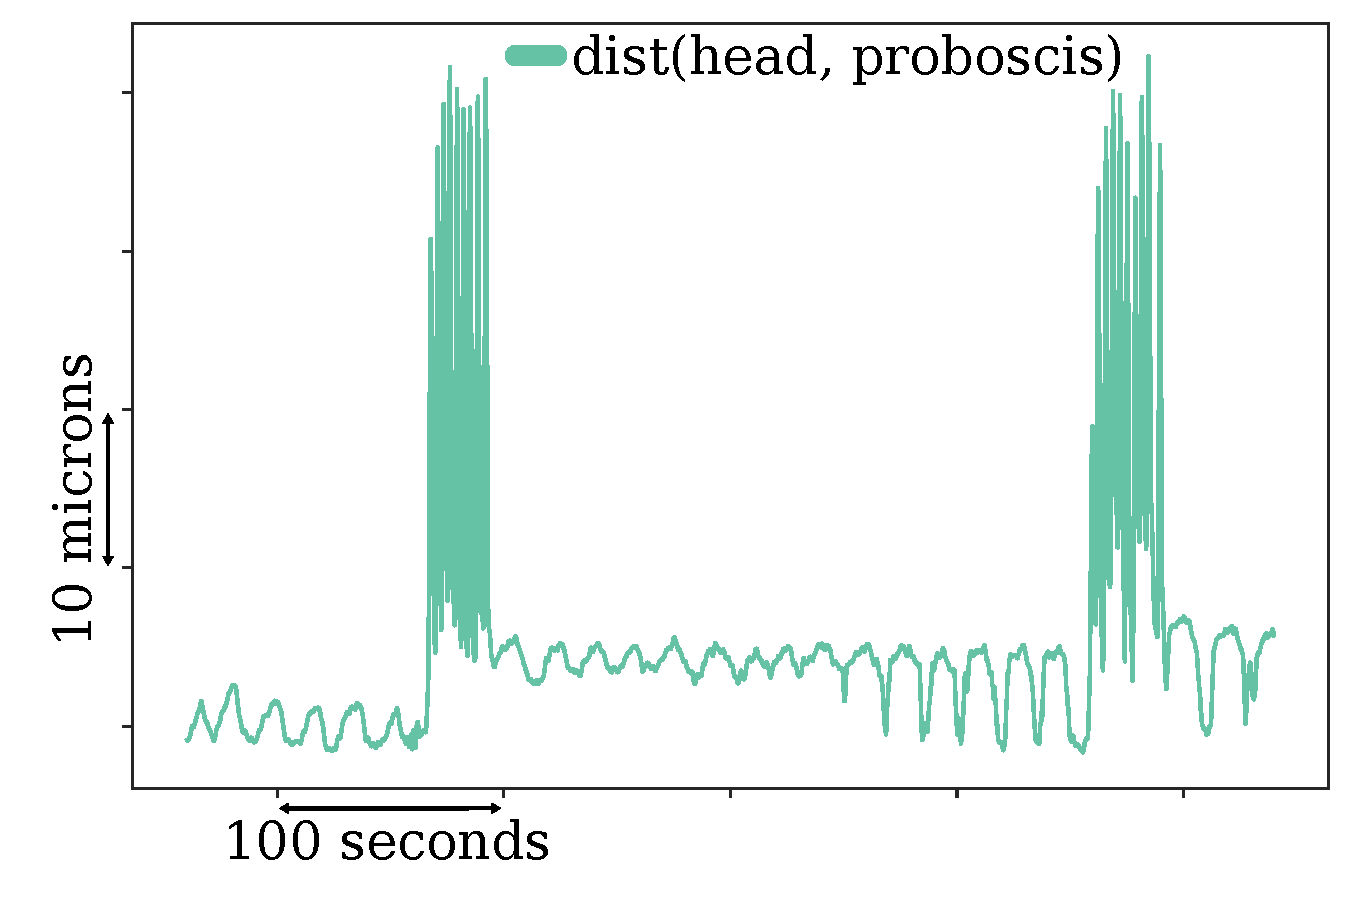
\includegraphics[width=\linewidth]{figures/ExampleTrajectory-ProboscisPumping.pdf}
		\caption{Pumping-like movement of the proboscis.}
	\end{subfigure}%
	\hfill
	\centering
	\begin{subfigure}[ht!]{0.32\linewidth}
		\centering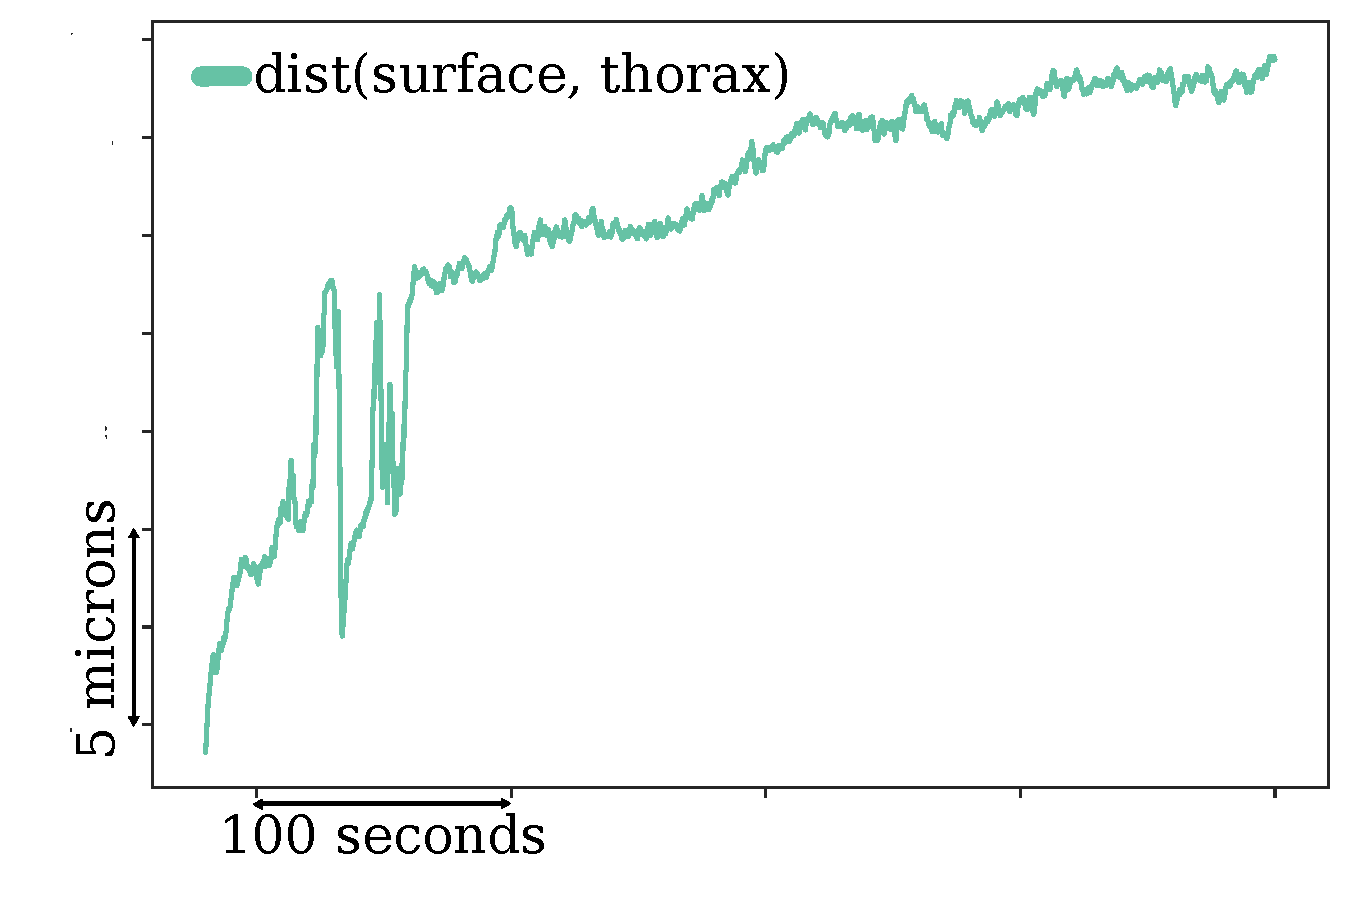
\includegraphics[width=\linewidth]{figures/ExampleTrajectory-PosturalAdjustment.pdf}
		\caption{Postural adjustment and movement of the thorax.}
	\end{subfigure}%
	\hfill
	\centering
	\begin{subfigure}[ht!]{0.32\linewidth}
		\centering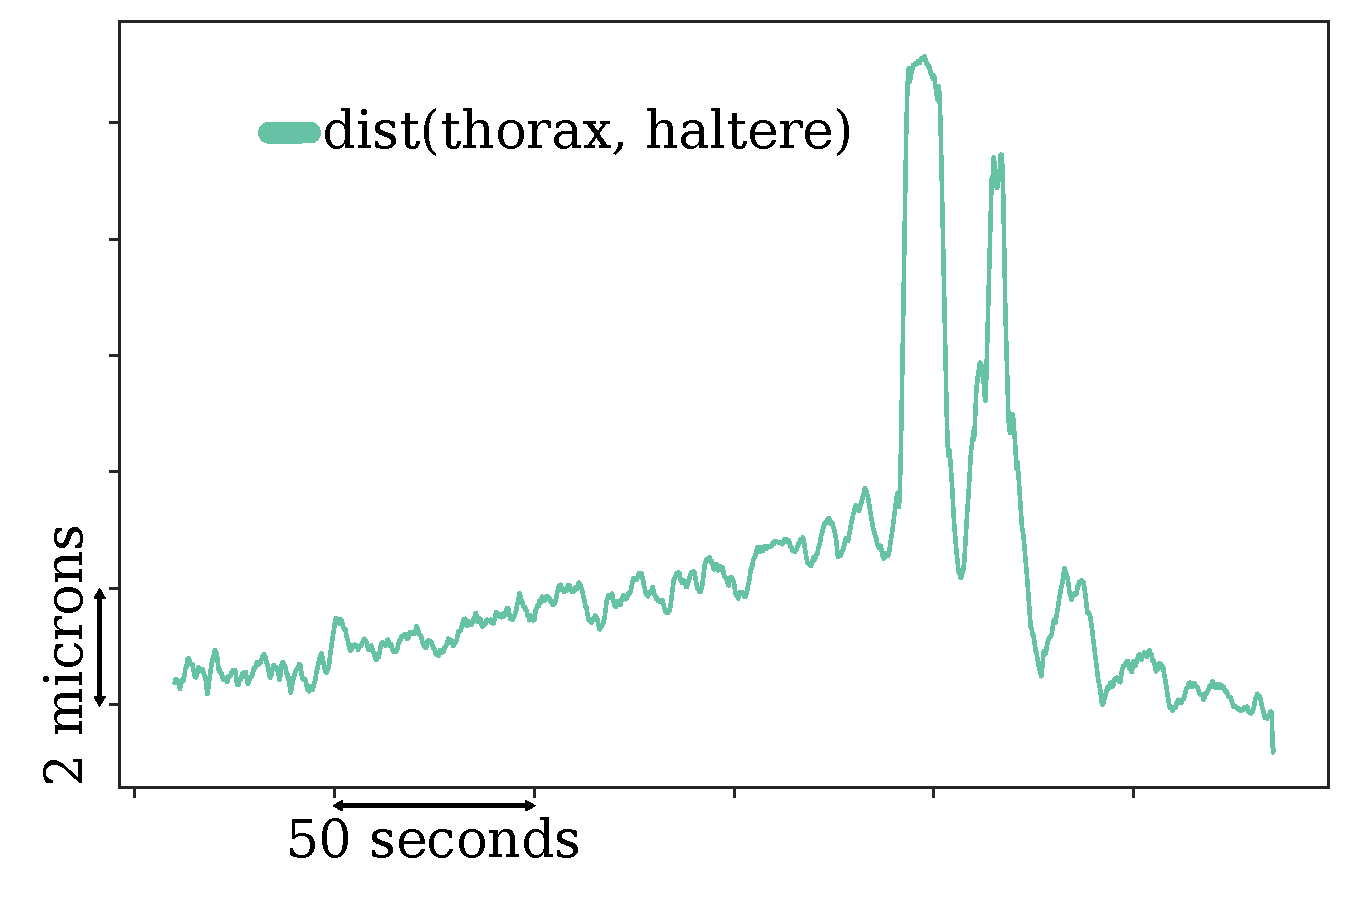
\includegraphics[width=\linewidth]{figures/ExampleTrajectory-HaltereSwitch_3.pdf}
		\caption{Switch-like movement of the haltere.}
	\end{subfigure}%
	\caption{Three spatio-temporal feature examples describing kinematics of different behaviors.}
\end{figure}

\subsection{Joint Angles Between Body Parts}
Given a triplet of body parts $\rbr{i,j,k}$, the angle between $i$ and $k$ around $j$ is calculated using the two-argument $\operatorname{arctangent}$ function as given below,
\begin{equation}
	\omega^{i,j,k}_t = \mathop{\rm{atan2}} \rbr{\det \begin{bmatrix} x_{i,t} - x_{j,t}, x_{k,t} - x_{j,t} \\ y_{i,t} - y_{j,t}, y_{k,t} - y_{j,t} \end{bmatrix}, \begin{bmatrix} x_{i,t} - x_{j,t} \\ y_{i,t} - y_{j,t} \end{bmatrix} \cdot \begin{bmatrix} x_{k,t} - x_{j,t}  \\ y_{k,t} - y_{j,t} \end{bmatrix}} + \pi.
\end{equation}

Then, similar to the change of distance features, the angular velocities are approximated by
\begin{equation}
	\dot{\omega}^{i,j,k}_t = \begin{cases} \frac{\abs*{\omega^{i,j,k}_{t+1} - \omega^{i,j,k}_{t}}}{\Delta t} & \textnormal{if } $t=0$ \textnormal{ or } $t=T$, \\ \frac{\abs*{\omega^{i,j,k}_{t+1} - \omega^{i,j,k}_{t-1}}}{2\Delta t} & \textnormal{otherwise}. \end{cases}
\end{equation}

\subsection{Cartesian Pose Values of Body Parts}
Cartesian pose values of a body part $i$ are straightforwardly given by the $x$ and $y$ coordinate values as follows:
\begin{equation}
	\begin{aligned}
		x^{i}_t & = x_{i,t}, \\
		y^{i}_t & = y_{i,t}.
	\end{aligned}
\end{equation}

Note that for a single body part, two feature values are generated.
Corresponding gradient features, namely the body part velocities along each cartesian component, are computed by
\begin{equation}
	\begin{aligned}
		\dot{x}^{i}_t & = \begin{cases} \frac{x^{i}_{t+1} - x^{i}_{t}}{\Delta t} & \textnormal{if } $t=0$ \textnormal{ or } $t=T$, \\ \frac{x^{i}_{t+1} - x^{i}_{t-1}}{2\Delta t} & \textnormal{otherwise}, \end{cases} \\
		\dot{y}^{i}_t & = \begin{cases} \frac{y^{i}_{t+1} - y^{i}_{t}}{\Delta t} & \textnormal{if } $t=0$ \textnormal{ or } $t=T$, \\ \frac{y^{i}_{t+1} - y^{i}_{t-1}}{2\Delta t} & \textnormal{otherwise}. \end{cases}
	\end{aligned}
\end{equation}

In order to compute overall two-dimensional velocity of a body part, one can always use the distance between the origin and corresponding body part.

\subsection{Constructing Spatio-temporal Feature Matrices}
Let $\mathcal{C}, \mathcal{D}$, and $\mathcal{A}$ denote the sets of body parts, body part pairs, and body part triplets; respectively defining cartesian pose values, distances, and angles.
Similarly, let $\mathcal{C}^{\prime}, \mathcal{D}^{\prime}$, and $\mathcal{A}^{\prime}$ denote sets that define sets of respective gradient features.
Then snapshot feature matrix $S$ constructed as follows;
\begin{equation}
	\V{S} = \rbr{\qmatrix{\rbr{\V{x}^i}_{i \in \mathcal{C}}} \concat \qmatrix{\rbr{\V{y}^i}_{i \in \mathcal{C}}} \concat \qmatrix{\rbr{\V{d}^{i,j}}_{\set{i,j} \in \mathcal{D}}} \concat \qmatrix{\rbr{\V{\omega}^{i,j,k}}_{\set{i,j,k} \in \mathcal{A}}}},
\end{equation}
where the vectors are defined as $\V{x}^{i}{=}\qmatrix{x^{i}_1, \cdots, x^{i}_T}$, $\V{y}^{i}{=}\qmatrix{y^{i}_1, \cdots, y^{i}_T}$,   $\V{d}^{i,j}{=}\qmatrix{d^{i,j}, \cdots, d^{i,j}_T}$, and $\V{\omega}^{i,j,k}{=}\qmatrix{\omega_1^{i,j,k}, \cdots, \omega^{i,j,k}_T}$.

Similarly, for gradient features, the feature matrix is constructed by concatenating change of distances, angular velocities and body part velocities; given by
\begin{equation}
	\V{G} = \rbr{\qmatrix{\rbr{\V{\dot{x}}^i}_{i \in \mathcal{C}^{\prime}}} \concat \qmatrix{\rbr{\V{\dot{y}}^i}_{i \in \mathcal{C}^{\prime}}} \concat \qmatrix{\rbr{\V{\dot{d}}^{i,j}}_{\set{i,j} \in \mathcal{D}^{\prime}}} \concat \qmatrix{\rbr{\V{\dot{\omega}}^{i,j,k}}_{\set{i,j,k} \in \mathcal{A}^{\prime}}}},
\end{equation}
where the vectors are defined as $\V{\dot{x}}^{i}{=}\qmatrix{\dot{x}^{i}_1, \cdots, \dot{x}^{i}_T}$, $\V{\dot{y}}^{i}{=}\qmatrix{\dot{y}^{i}_1, \cdots, \dot{y}^{i}_T}$,   $\V{\dot{d}}^{i,j}{=}\qmatrix{\dot{d}^{i,j}, \cdots, \dot{d}^{i,j}_T}$, and $\V{\dot{\omega}}^{i,j,k}{=}\qmatrix{\dot{\omega}_1^{i,j,k}, \cdots, \dot{\omega}^{i,j,k}_T}$.

The resulting two feature matrices are $\V{S} \in \mathbb{R}^{T \times \rbr{2\card*{\mathcal{C}}+\card*{\mathcal{D}}+\card*{\mathcal{A}}}}$, namely snapshot feature matrix, and $\V{G} \in \mathbb{R}^{T \times \rbr{2\card*{\mathcal{C}^{\prime}}+\card*{\mathcal{D}^{\prime}}+\card*{\mathcal{A}^{\prime}}}}$, namely gradient feature matrix.
Let $N_S$ denote the number of snapshot features, being equal to $2\card*{\mathcal{C}}+\card*{\mathcal{D}}+\card*{\mathcal{A}}$ and let $N_G$ denote the number of gradient features, which is equal to $2\card*{\mathcal{C}^{\prime}}+\card*{\mathcal{D}^{\prime}}+\card*{\mathcal{A}^{\prime}}$.

\section{Computation of Dynamic Postural Features}\label{section:dynamic-postural-features}
Instantaneous values of spatio-temporal features do not provide a sufficient description of complex postural dynamics of behaviors.
Understanding the output of a complex biological system, in our case behavior, can only be achieved by studying multiple time-scales together.
Previous studies attempt to search behavioral motifs, e.g., repeated sub-sequences of actions with finite length, within the behavioral time series \citep{ye_time_2011, brown_dictionary_2013}.
However, as \citet{berman_mapping_2014} states, this paradigm usually requires problems of temporal alignment and relative phasing between different scales.
Alternatively, extending spatio-temporal features to capture postural dynamics at different time-scales eliminate requirements of temporal alignment and motif based analysis.
In order to extend the spatio-temporal features to dynamic postural features, we applied wavelet transformation (similar to \citet{berman_mapping_2014}) and computed moving statistics at different time-scales (similar to \citet{kabra_jaaba_2013}), respectively for the snapshot feature set ($\V{S}$) and the gradient feature set ($\V{G}$).

\subsection{Moving Statistics of Gradient Features}
Gradient features only reflect the instantaneous values of velocities with respect to the sampling rate.
In order to capture how these values change within a given interval, the moving statistics, e.g., mean and standard deviation, of gradient features are computed with a sliding window approach.
Let $\tau$ be the window size parameter, i.e., the timescale of interest, then the moving mean of the corresponding gradient feature $\V{g}_{i}$ is given by the function $\mu_\tau$:
\begin{equation}
	\mu_{\tau}(g_{i,t}) = \sfrac{1}{\min\{t+\tau,\, T\}-\max\{t-\tau,\, 1\}+1} \sum_{t^{\prime}=\max\{t-\tau,\, 1\}}^{\min\{t+\tau,\, T\}} g_{i, t^{\prime}}.
\end{equation}

Similarly, the moving standard deviation of a gradient feature $g_{i,t}$ by is computed by $\sigma_\tau$, as in the below equation.
\begin{equation}
	\sigma_\tau(g_{i,t}) = \rbr{\sfrac{1}{\min\{t+\tau,\, T\}-\max\{t-\tau,\, 1\}+1} \sum_{t^{\prime}=\max\{t-\tau,\, 1\}}^{\min\{t+\tau,\, T\}} \rbr{\mu_{\tau}(g_{i,t}) - g_{i, t^{\prime}}}^2}^{\sfrac{1}{2}}
\end{equation}

Moving statistics feature generation approach is used to learn animal behavior by \citet{kabra_jaaba_2013}, and \citet{marshall_continuous_2021} is also included such features into the analysis.

\subsection{Wavelet Transformation of Snapshot Features}
The wavelet domain is a useful representation of postural dynamics due to the following reasons given by \citet{berman_mapping_2014}, and the proposed spectrogram generation is used by others as well \citep{marshall_continuous_2021, todd_systematic_2017}.
\begin{itemize}
	\item It describes dynamics over multiple time-scales simultaneously by possessing a multi-resolution time-frequency trade-off.
	\item It eliminates the requirement of precise temporal alignment for capturing periodic behaviors by taking amplitudes of the continuous wavelet transform of each snapshot feature at different scales.
\end{itemize}
Given a function $s(t)$, continuous wavelet transformation at a frequency $f>0$ is expressed as the following integral:
\begin{equation}
	W_{f,t^{\prime}}\qmatrix{s\rbr{t}} = \frac{1}{\sqrt{a\rbr{f}}} \int_{-\infty}^{\infty} s\rbr{t} \Psi^\ast\rbr{\frac{t - t^{\prime}}{a(f)}} \dd{t},
\end{equation}
where $\Psi$ is the wavelet function and $a$ is a function for converting frequencies to wavelet scale factor.
The Morlet wavelet is suitable for describing postural dynamics which is closely related to human perception, both hearing and vision \citep{daugman_uncertainty_1985}, and is used in the pipeline.
The corresponding wavelet function is given by
\begin{equation}
	\Psi(t) = \exp{\frac{t^2}{2}} \cos(w_0t),
\end{equation}
where $w_0$ is a non-dimensional parameter. The frequency-to-scale conversion function $a$ for the Morlet wavelet is as follows:
\begin{equation}
	a\rbr{f} = \frac{w_0 + \sqrt{2+w_0^2}}{4 \pi f}.
\end{equation}

For the discrete sequence of snapshot feature $\V{s}_i$ with sampling period $\Delta t$, $W_{f,t^\prime}[s(t)]$ translates into
\begin{equation}
	\label{eq:wavelet-practical}
	W_f\rbr{\V{s}_i, t^\prime} = \frac{1}{\sqrt{a(f)}} \sum_{t=1}^{T} {\Delta t} s_{i,t} \Psi^\ast\rbr{\frac{t-t^{\prime}}{a{f}}},
\end{equation}
where $t^\prime, t \in \mathbb{Z}$ and $ 1 \leq t^\prime \leq T$ \citep{torrence_practical_1998}.

\subsubsection{Normalization of Wavelet Power Spectrum}
In order to ensure that wavelet transforms (Equation~\ref{eq:wavelet-practical}) at each frequency $f$ are directly comparable to each other and to the other transformed time series, the transformation $W_f$ has to be normalized at each frequency $f$ to have unit energy.
This normalization for the Morlet wavelet at frequency $f$ is as follows:
\begin{equation}
	C(f) = \frac{\pi^{-\frac{1}{4}}}{\sqrt{2a(f)}}\exp{\sfrac{1}{4}\rbr{w_0-\sqrt{w_0^2+2}}^2}.
\end{equation}
So resulting normalized transformation, which is also used to generate the spectrogram in \citet{berman_mapping_2014}, is given by
\begin{equation}
	W^0_f\rbr{\V{s}_i, t^\prime} = \frac{1}{C\rbr{f}} \abs*{W_f\rbr{\V{s}_i, t^\prime}}.
\end{equation}

In addition to the above conventionally used normalization, we alternatively adopted the normalization proposed by \citet{liu_rectification_2007}. According to this alternative adjustment, the wavelet power spectrum should be equal to the transform coefficient squared divided by the scale it associates.
\begin{equation}\label{equation:wavelet-normalization}
	W^{0}_f\rbr{\V{s}_i, t^\prime} = \frac{W_f\rbr{\V{s}_i, t^\prime}^2}{a\rbr{f}}
\end{equation}
We observed substantial improvements using this power spectrum.

\subsubsection{Determining Spectrum Frequencies}
We investigate two different approaches for computing a set of frequencies and, we include both of them in the behavior mapping pipeline.
One set is dyadically spaced frequencies between $f_{\textnormal{min}}$ and $f_{\textnormal{max}}$ via
\begin{equation}\label{equation:dyadically-spaced-spectrum}
	f_i = f_{\textnormal{max}} 2^{-\frac{i-1}{N_f-1}\log{\frac{f_{\textnormal{max}}}{f_{\textnormal{min}}}}},
\end{equation}
where $f_{\textnormal{max}} = \sfrac{FPS}{2} \textnormal{ Hz}$ is the Nyquist frequency.

The other alternative set of frequencies is linearly spaced between $f_{\textnormal{min}}$ and $f_{\textnormal{max}}$ by
\begin{equation}
	f_i = f_{\textnormal{min}} + \frac{f_{\textnormal{max}} - f_{\textnormal{min}}}{N_f-1}i,
\end{equation}
for $i=1,2,\dots,N_f$, and their corresponding wavelet scales are computed by $a\rbr{f_i}$.

\subsection{Constructing Dynamic Postural Feature Tensors}
Let $\mathcal{T}_S=\set{\sfrac{1}{f_{\textnormal{min}}}, \cdots \sfrac{1}{f_{\textnormal{max}}}}$ and $\mathcal{T}_G=\set{\tau_{\textnormal{min}}, \cdots, \tau_{\textnormal{max}}}$ denote the time-scale sets respectively for wavelet transforms of snapshot features and moving statistics of gradient features. Then corresponding feature tensors are given as follows:
\begin{equation}
	\begin{aligned}
		\V{W}        & = \rbr{W^0_{f}\rbr{\V{s}_i, t}}_{1 \leq t \leq T, \, \sfrac{1}{f} \in \mathcal{T}_S, \, 1 \leq i \leq N_S}, \\
		\V{M}^\mu    & = \rbr{\mu_\tau\rbr{g_{i,t}}}_{1\leq t \leq T, \, \tau \in \mathcal{T}_G, \, 1 \leq i \leq  N_G},           \\
		\V{M}^\sigma & = \rbr{\sigma_\tau\rbr{g_{i,t}}}_{1\leq t \leq T, \, \tau \in \mathcal{T}_G, 1 \leq i \leq N_G}.
	\end{aligned}
\end{equation}

The resulting extended feature tensors of dynamic postural representations are $\V{W} \in \mathbb{R}^{T \times \card*{\mathcal{T}_s} \times N_S}$, $\V{M}^\mu \in \mathbb{R}^{T \times \card*{\mathcal{T}_v} \times N_G}$ and $\V{M}^\sigma \in \mathbb{R}^{T \times \card*{\mathcal{T}_v} \times N_G}$.

\section{Computation of Behavioral Representations}
After applying wavelet transformation or computing moving statistics to extend extracted spatio-temporal features to dynamic postural features, a couple of additional operations are required to continue in the behavior mapping pipeline.

\subsection{Flattening Dynamic Postural Feature Tensors}
As constructed in Section~\ref{section:dynamic-postural-features}, dynamic postural feature tensors are $\V{W} \in \mathbb{R}^{T \times \card*{\mathcal{T}_S} \times N_S}$, $\V{M}^\mu \in \mathbb{R}^{T \times \card*{\mathcal{T}_G} \times N_G}$, and  $\V{M}^\sigma \in \mathbb{R}^{T \times \card*{\mathcal{T}_G} \times N_G}$.
In order to apply manifold learning-based dimensionality reduction algorithms or traditional machine learning algorithms such as decision trees, the last two dimensions of these feature tensors need to be flattened.
As a result, feature matrices are $\V{\tilde{W}} \in \mathbb{R}^{T \times \rbr{ N_S\card*{\mathcal{T}_S}}}, {\V{\tilde{M}}^\mu} \in \mathbb{R}^{T \times \rbr{ N_G\card*{\mathcal{T}_G}}}$ and ${\V{\tilde{M}}^\sigma} \in \mathbb{R}^{T \times \rbr{ N_G\card*{\mathcal{T}_G}}}$ are obtained.

\subsection{\texorpdfstring{$\textnormal{L}_1$}{L1} Normalization of Features}\label{section:feature-normalization}
Dynamic postural feature distributions of similar behaviors may differ among flies due to different characteristics such as gender, and being sleep-deprived.
Due to the two-dimensional nature of the video recordings, different orientations may cause observing different feature values for the same behavior.
In order to have a homogeneous feature space among flies and along the time, at each time step $t$, $\textnormal{L}_1$ normalization is applied as follows:
\begin{equation}
	\V{\hat{w}}_i = \rbr{\frac{\tilde{w}_{t,i}}{\sum_{j=1}^{N_S \card*{\mathcal{T}_s}}\tilde{w}_{t, j}}}_{1 \leq t \leq T} \dband \V{\hat{W}}   = \qmatrix{\rbr{\V{\hat{w}}_i}_{1 \leq i \leq N_S\card*{\mathcal{T}_S}}}.
\end{equation}
Similarly, $\textnormal{L}_1$ normalized versions of ${\V{\tilde{M}}^\mu}$ and ${\V{\tilde{M}}^\sigma}$, namely $\V{\hat{M}}^\mu$ and $\V{\hat{M}}^\sigma$ are obtained.
Here $\V{\hat{W}}$, $\V{\hat{M}}^\mu$ and $\V{\hat{M}}^\sigma$ are the final multivariate time series of normalized high dimensional behavioral representation of a single experiment data, i.e., single fruit fly recorded between ZT10 and ZT2.
Notice that we may treat each time step, that is, the frame, as a discrete probability distribution after $\textnormal{L}_1$ normalization.
